As the name suggests, this chapter has a different focus compared to the previous ones. This chapter is concerned with classifying a few games, both in terms of gameplay and in terms of algebraic structure. This is relevant because it highlights important characteristics in underlying structure and in possible values.

This sections features a few theorems that end up proving an upper bound for the boiling point of classes of games, called here \textit{the result}.

\subsection*{Some more thermograph characteristics}

The temperature's upper bound results from a thorough analysis of the thermograph. The paper \textit{Bounding Game Temperature Using Confusion
Intervals} \cite{12} brings the first of such results, although the content featured first in Svenja Huntemann's PhD thesis \cite{5} in 2018, a year before. The proof of the boiling point requires a few smaller results and all the required content is summarized in the remaining of this subsection.

The confusion interval of a game is the range of numbers with which it is confused. A game is confused with a number if it is neither greater, smaller nor equal to that number. Any game with temperature greater than 0 is confused with numbers. Take any instance of such cases from previous sections to verify that their confusion interval includes all numbers between the points where the thermograph intersects the $t=0$ line. Some intervals also include either one or both of the intersection points, depending on what the toenail of the thermograph looks like.

However, the reader can also verify that some non-numbers with temperature 0 are also confused with numbers. Section four shows that the thermograph of \gam{0}{0} is different to that of 0, although above $t=0$ they are the same. However, if using the surreal $\leq$ operation defined in \textit{Chapter 3}, one notices that $\gam{0}{0} \not\lessgtr 0$, which shows $0$ is confused with \gam{0}{0}. However, not all non-numbers behave this way, because some fall in gaps, not being confused with any number. Gaps is another delicate subject related to numbers that will not be discussed. \gam{0}{\gam{0}{0}} is a game inside a gap.

The confusion interval of a game \Gm{} is usually indicated by $\ell(G)$ and the points where the left and right trajectories, $\lambda_t(G), \rho_t(G)$, intersect the $t=0$ line, are usually denoted by $LS(G)$ and $RS(G)$, and called left and right stops. Therefore $\ell(G) = LS(G)-RS(G)$. Another important definition is the thermic version of a game. A thermic version of a game \Gm{} is a game $\tilde{\Gm{}}$ with the same temperature of \Gm{} but with only one left and one right option, that are also left and right options for \Gm{}.

The existence of thermic versions follows: if \Gm{} is hot, then there exists left and right options of \Gm{}, \Gm{^{L_*}} and \Gm{^{R_*}}, such that \mbox{$t(G) = t(\gam{\Gm{^{L_*}}}{\Gm{^{R_*}}})$}. The proof is simple. The mast of \Gm{} begins where the cooled thermographs of some of the left and right options first intersect. There are possibly many left and right options that intersect on the same point. By taking any one of them, \Gm{^{L_+}} and \Gm{^{R_+}}, it is clear that the thermic version of a game exists, because $t(G) = t(\gam{\Gm{^{L_+}}}{\Gm{^{R_+}}})$.

Finding in practice the thermic version of a game is not at all simple. In fact, without additional information of \Gm{}, it would be needed to build the entire thermograph, or equivalent information, beforehand. This is an important consideration, that is also made on Huntemann's thesis, but one that is not problematic. Soon, the bound will be created for \Gm{} directly, so that finding the thermic version is not necessary.

It is trivial but it is worth highlighting that the thermograph of \Gm{} and that of $\tilde{\Gm{}}$ may not be the same. In particular $\lambda_t(\tilde{\Gm{}}) \ge \lambda_t(\Gm{})$ and $\rho_t(\tilde{\Gm{}}) \leq \rho_t(\Gm{})$. If it is not clear why the observation is true: for any temperature $t$, the trajectories of the thermograph were either the maximum/minimum of all the corresponding options. The selected left and right options for the thermic version of \Gm{} are only the minimum/maximum for temperatures close to the boiling point. Therefore the initial part of the trajectory might be different, but is always lesser/greater or equal to the thermic trajectories.

Using the notation built so far it may be simpler. $\lambda_t(\Gm{}) = LS(\Gm{_t})$ and, by definition, $\lambda_t(\Gm{}) = max_{\Gm{^L}}(RS(\Gm{^L_t}) - t)$. Since $\Gm{^{L_+}} \in \Gm{^L}$, it is clear that $\lambda_t(\tilde{\Gm{}}) \ge \lambda_t(\Gm{})$. An equivalent statement can be made for the right trajectory.

A result, when taking $t=0$, is:

\begin{align*}
\ell(\tilde{\Gm{}}) \leq& \ell(\Gm{})\\
\text{Since } \ell(\tilde{\Gm{}}) = LS(\tilde{\Gm{}}) - RS(\tilde{\Gm{}})\leq& LS(\Gm{}) - RS(\Gm{}) = \ell(\Gm{})
\end{align*}

The thermograph, as described in the previous section, is composed of straight lines and $\pm 45 \deg$ oblique lines. The bound is based on this and the size of the confusion interval. Before proceeding, one additional definition.

Let $T^L$ be the sequence $(0, t_1, t_2, \ldots, t_k)$ of the temperatures of the turning points of $\lambda(\tilde{\Gm{}})$. Let, now, $A^L$ be the sequence $(a_0, a_1, \ldots, a_k)$ of labels given by:

\hspace{2cm}$
\begin{cases}
a_i $ is \textit{vertical} if $ \rho(\tilde{\Gm{}}^L_{t_{i+1}}) = \rho(\tilde{\Gm{}}^L_{t_i})\\
a_i $ is \textit{oblique} if $ \rho(\tilde{\Gm{}}^L_{t_{i+1}}) < \rho(\tilde{\Gm{}}^L_{t_i})
\end{cases}
$

Lastly,

\hspace{2cm} $T^L_{\text{V}} = \sum\limits_{\substack{i\;|\;a_i \text{ is} \\ \text{vertical}}}(t_{i+1} - t_i)$

\hspace{2cm} $T^L_{\text{O}} = \sum\limits_{\substack{i\;|\;a_i \text{ is} \\ \text{oblique}}}(t_{i+1} - t_i)$

Notice that the right counterpart can be done similarly. Let $T^L_{\text{V}}$ be the length of the vertical segments and let $T^L_{\text{O}}$ be the length of the oblique segments. The temperature of the game \Gm{} can be given by a combination of the oblique and vertical parts of the thermograph like the following:

$$
	t(\Gm{}) = T^L_{\text{V}} + T^L_{\text{O}}
$$
\newpage
The length of the confusion interval of the thermic version of \Gm{} can also be given in terms of the oblique part of the thermograph:

$$
\ell(\tilde{\Gm{}}) = T^L_{\text{O}} + T^R_{\text{O}}.
$$

\subsection*{The theorem}

\textit{The theorem} discussed in the beginning of the chapter is the following:

For any game \Gm{} and $\tilde{\Gm{}}$ its thermic version, it is true that


\begin{align*}
	t(\Gm{}) &\leq \ell(\Hm) + \frac{\ell(\Gm{})}{2} \\
	& \\
	\text{Where } &\begin{cases}
		\small
		\Hm = \tilde{\Gm{}}^L &\text{if } T^L_V \ge T^R_V \\
		\Hm = \tilde{\Gm{}}^R &\text{otherwise} \\
	\end{cases}
\end{align*}

For simplicity, the proof considers that $\Hm = \tilde{\Gm{}}^L$, but again, an equivalent procedure proves the other case.

The length of $T^L_V$ is at most the length of the oblique segments of $\rho(\tilde{\Gm{}}^L)$. Notice that it could be smaller because the left and right options might intersect before the mast of $\tilde{\Gm{}}^L$. In any case, it is clear that the length of this oblique segment is at most the same size of the confusion interval of $\tilde{\Gm{}}^L$. It could be smaller in case there are oblique segments in $\lambda(\tilde{\Gm{}}^L)$.

Therefore, $T^L_V \leq \ell(\tilde{\Gm{}}^L)$

Additionally, it is true that:

$$
T^L_V + T^L_O = T^R_V+T^R_O
$$

And, since in this case $T^L_V \ge T^R_V$:

$$
T^L_O \leq T^R_O
$$

Therefore:

\begin{align*}
	2\times T^L_O &\leq T^L_O + T^R_O \\
	&= \;\ell(\tilde{\Gm{}})\\
	&\leq \ell(\Gm{})\\
	T^L_O \leq\; &\frac{\ell(\tilde{\Gm{}})}{2} \leq \frac{\ell(\Gm{})}{2}
\end{align*}

Resulting in:

$$
t(G) = T^L_V + T^L_O \leq \ell(\tilde{\Gm{}}^L) + \frac{\ell(G)}{2}
$$

$T^L_V + T^L_O =\;T^R_V+T^R_O$ is straight forward, because what defines the height is the intersection point of left and right, which is the same for both trajectories. $2\times T^L_O \leq T^L_O + T^R_O$ is a direct result of the previous equation with the given consideration that $T^L_V \ge T^R_V$. 

Although longer than other proofs in this text, it is yet another simple proof. The equations and the many symbols might make it unclear, but each of the steps are short and can be visualized.

This theorem uses the thermic version of games, which, again, are hard to find in itself. However, from this version, another result that does not use the thermic versions is possible.

\textit{The theorem} might be re-written as:

Let $n, m$ be two non-negative numbers. If $S$ is class of games such that for all $G \in S,\;\ell(G) \leq n$ and for left and right options \Gm{^{L/R}}, $\ell(G^{L/R}) \leq m$, then:

$$
BP(G) \leq \frac{n}{2} + m
$$

Although immediate, deciding whether the first version implies the version above might require an explanation. $t(G) \leq \ell(\tilde{\Gm{}}^L) + \frac{\ell(G)}{2} \leq \frac{n}{2} + \ell(\tilde{\Gm{}}^L)$ because for all \mbox{$\Gm{} \in S$}, \mbox{$\ell(G) \leq n$}. Since $\ell(G^{L/R}) \leq m$, then $\ell(\tilde{\Gm{}}^L) \leq m$, which implies the last inequality \mbox{$t(G) \leq \frac{n}{2} + \ell(\tilde{\Gm{}}^L) \leq \frac{n}{2} + m$}.

Handling a class of games is not as straight-forward as using the definitions typically used in this text. A good way to use the theorem is to first create a class, based the restrictions - therefore having a bound for the confusion intervals of the games and its Left and Right options. Then one should prove a game or a pattern of games belongs to this class, to make use of this bound.

Let, for example, the class $S$ to be defined by $\{G : \ell(G)\leq100, \ell(G^L)\leq200, \ell(G^R)\leq200\}$. Since $S$ meets the requirements it has the proposed boiling point. For all games $G \in S, BP(G) \leq 250$. The maximum length of the confusion intervals are so large that, in particular, all games of this text belong to $S$. The hottest game \Gm{} analyzed in this text is:

\begin{center}
	\begin{tikzpicture}
		\begin{scope} []
			\draw[fill=yellow] (-1,-1) rectangle ++(8,1.9);
			\node[circle, draw, fill=purple2] at (0,0) {7 $|$ {-}9};
			\node[circle, draw, fill=purple2] at (2,0) {28 $|$ {-}4};
			\draw[thick] (3,-0.75) -- (3,0.75);
			\node[circle, draw, fill=purple2] at (4,0) {{-}3 $|$ 1};
			\node[circle, draw, fill=purple2] at (6,0) {2 $|$ 22};
		\end{scope}
	\end{tikzpicture}
\end{center}

The thermograph of \Gm{=\gam{\gam{7}{9},\gam{28}{4}}{\gam{-3}{-1},\gam{2}{-22}}} is:
\begin{center}
	\includegraphics[scale=0.5]{../images/thermA.png}
\end{center}

In this case, $\ell(G) = 10 \leq 100$ and \mbox{$\ell(\gam{7}{9}) = \ell(\gam{-3}{-1}) = 0 \leq 200$} and, finally, \mbox{$\ell(\gam{28}{4}) = \ell(\gam{2}{-22}) = 24 \leq 200$}, so \Gm{\in S}. The boiling point bound the theorem provided for $S$ is loose for \Gm{}, since $\forall H \in S, BP(H) \leq 250$ and $BP(G) = 13$. However, the size of the confusion intervals that defined the class are also loose. In general cases, specially when confusion intervals start getting large, the bound will be loose, but that is because the bound itself is large, not because the theorem is inefficient.

Let $S_*$, now, be the class given by $\{G : \ell(G)\leq10, \ell(G^L)\leq24, \ell(G^R)\leq24\}$. From the analysis of the previous paragraph, \Gm{\in S_*}. However, in this case, the confusion intervals of \Gm{} are tight in respect to the ones that define the class. From \textit{the theorem} for all games $G \in S_*,\; BP(G) \leq 29$. The bound is tighter for \Gm{} but is still loose, which may lead to the belief that this bound is loose in general.

In order to verify whether the bound is in fact loose, it would be required to show the following, or something similar:
$$
\forall S,\;\exists x\in \mathbb{R}\footnotemark,\; x>0\;|\; \underset{G\in S}{\max}BP(G) + x \leq BP(S)
$$

\footnotetext{Convergence can be more complicated using surreal numbers. If instead $x\in\textup{SN}$ was used, an additional infinitesimal $y\in\textup{SN}$ would be required resulting in additional complexity in a topic that is not the focus of the text.}

To dismiss that idea, however, it could be shown:
$$
\exists G \in S_*\;|\;\not\exists x \in \mathbb{R}, x>0,\; BP(G) + x \leq BP(S)
$$

Starting out with the previous example, take $\tilde{G} = \gam{\gam{28}{4}}{\gam{2}{-22}}$. The temperature is 13, the same as before, since, $t(\Gm{}) = \tilde{t(\Gm{})}$. However, the Left and Right slant may be moved, since $\ell(\tilde{G}) = 2$. Take \Gm{_+=\gam{\gam{36}{12}}{\gam{2}{-22}}}, result of shifting the left slant to the left, which maintains the left and right confusion intervals, but increases the confusion interval for $\tilde{\Gm{}}$ while maintaining that \Gm{_+ \in S_*}.

\begin{center}
\begin{tabular}{cc}
\includegraphics[scale=0.5]{../images/gtherm.png} & \includegraphics[scale=0.5]{../images/gplus.png} \\
$\tilde{G}$ & \Gm{_+} \\
\end{tabular}
\end{center}

The temperature 17 is higher than the initial one but is still far away from the desired 29. However, it is still possible to increase it more. The boiling point of left and right slants are 12, and, for this reason, the oblique line in the thermograph start at $t=12$. Making the left and right games hotter would increase the overall temperature, but increasing the confusion interval is not allowed as it is desired that the resulting game belongs to the class $S_*$.

Since the thermographs of \Gm{_+^{L/R}} below the boiling point are made of two oblique lines, making part of the lines straight would increase their temperature. The way to achieve higher temperature without increasing the confusion interval is changing \Gm{_+^{L}} so that $RS(G_+^{L})$ remains in the same position but $T^R_O$ of \Gm{_+^L} is increased. Change, then \Gm{_+^L} to \gam{\gam{60}{36}}{12} and \Gm{^R} to \gam{2}{\gam{-22}{-46}}. The reason why \gam{36}{12} was replaced by \gam{60}{\gam{36}{12}} as \Gm{^L} is to keep $\ell(H) = 24$, for $H$ any hot game in the left and right sub-trees of the game tree of $G_+$. This pattern will be kept and helps simplifying results.

Let \Gm{_-=\gam{\gam{\gam{60}{36}}{12}}{\gam{2}{\gam{-22}{-46}}}} be the game resulting from this changes. The temperature of \Gm{_-} is 23. To simplify further analysis, take a game \Gm{_1}, result of centering \Gm{_-} at 0. In this case, \Gm{_1 = \gam{\gam{\gam{53}{29}}{5}}{\gam{{-}5}{\gam{-29}{-53}}}}.  Notice that \Gm{_1 = \pm\gam{\gam{53}{29}}{5}}.

\begin{center}
	\begin{tabular}{cc}
		\includegraphics[scale=0.5]{../images/gminus.png} & \includegraphics[scale=0.5]{../images/gone.png} \\
		\Gm{_-} & \Gm{_1} \\
	\end{tabular}
\end{center}

Using the strategy of making one of the slants of \Gm{^{L/R}} straighter in order to increase their temperature, it is possible to keep increasing the temperature of \Gm{}. Consider the following sequence of games is $S_*$:

\begin{center}
	\begin{tabular}{c|c|c}
		$i$ & \Gm{_i} & $t(G_i)$	\\[0.1cm]
		\hline
		0 & $\pm$ \gam{29}{5} & 17 \\[0.1cm]
		\hline
		1 & $\pm$ \gam{\gam{53}{29}}{5} & 23 \\[0.1cm]
		\hline
		2 & $\pm$ \gam{\gam{\gam{77}{53}}{29}}{5} & 26 \\[0.1cm]
		\hline
		3 & $\pm$ \gam{\gam{\gam{\gam{101}{77}}{53}}{29}}{5} & 27.5 \\
	\end{tabular}\\
	\vspace{0.3cm}$\cdots$
\end{center}

The result that the temperature of games in this sequence increases and converges to 29 is required to prove the bound is tight, so it must be proved. Instead of only proving the convergence in this particular case, which is is sufficient, the following proof shows that the boiling point, given by Svenja, for all classes are tight. The following proof is general for all sequence of games made in the likes of the sequence above.

\textit{Proof:}

Let $OB$ be the bound $\ell(G^{L/R})$ for the options of \Gm{} in the class $S$.

Let $B$ be the bound for $\ell(G)$ in the class $S$.

\begin{list}{}{}
	\item[$\rightarrow$] Both $T^L_V$ and $T^R_V$ of $G$ are given by 
	$$\sum_{i=0}^n\frac{OB}{2^{i+1}}$$
	The following proof only shows the case for the left option as the proof for the right is analogous.
	
	[Via induction on $i$]
	
	Base case: $n = 0$.
	
	In this case, $G_i^L = G_0^L = \gam{\frac{B}{2} + OB}{\frac{B}{2}}$. Since $G_0^L$ is a switch, both the trajectories are oblique. The trajectories, then, meet at $BP(G_0^L) = \frac{OB}{2}$. This way, the right trajectory of the thermograph of $G_0^L$ is oblique until $\frac{OB}{2}$ and vertical after that. Therefore the left trajectory of $G_0$ is vertical until $\frac{OB}{2}$ and oblique after that point.
	
	As a result, 
	$$T^L_V \text{ of } G = \frac{OB}{2} = \sum_{i=0}^0\frac{OB}{2^{i+1}}$$
	
	Considering now that $k > 0$.
	
	$$
	\Gm{_k=\gam{
			\gam{
				\gam{
					\gam{\ldots
						\gam
							{\frac{B}{2} + (k+1)OB}
							{\frac{B}{2} + kOB}
						}
						{\ldots}
					}
					{\frac{B}{2} + 2OB}
				}
				{\frac{B}{2}+OB}
			}
			{\frac{B}{2}}
		}
	$$
	
	Let $b = \frac{B}{2}+OB$. It is possible to rewrite $G$:
	
	$$
	\Gm{_k=\gam{
			\gam{
				\gam{
					\gam{\ldots
						\gam
						{b + kOB}
						{b + (k-1)OB}
					}
					{\ldots}
				}
				{b+OB}
			}
			{b}
		}
		{\frac{B}{2}}
	}
	$$
	
	Via inductive hypothesis on:
	
	$$
	\Hm{=
			\gam{
				\gam{
					\gam{\ldots
						\gam
						{b + kOB}
						{b + (k-1)OB}
					}
					{\ldots}
				}
				{b + OB}
			}
			{b}
	}
	$$
	
	The total vertical length of the left trajectory of $\Hm_* = \pm \Hm$ is equal to $\sum\limits_{i=0}^{k-1}\frac{OB}{2^{i+1}}$. Added to  the fact that the right option of $\Hm$ is a number, the total oblique length of the right trajectory of $\Hm^L$ is equal to $\sum\limits_{i=0}^{k-1}\frac{OB}{2^{i+1}}$ and it is oblique until the boiling point. 
	
	Because of this, the draft of the left trajectory of $G_k^L$ is vertical until the boiling point of $\Hm$. Since the right option of $G_k^L$ is a number, its right trajectory is oblique until the boiling point. Therefore, $BP(G_k^L) = \sum\limits_{i=0}^{k}\frac{OB}{2^{i+1}}$.
	
	Once again because the right slant of $G_k^L$ is oblique until $\sum\limits_{i=0}^{k}\frac{OB}{2^{i+1}}$, it is true that:
	
	$$
	T^L_V \text{ of } G = \sum\limits_{i=0}^{k}\frac{OB}{2^{i+1}}
	$$
	
	\item[$\rightarrow$] If both the left option of \Gm{^L} and the right option of \Gm{^R} have their straight length increased by $l$, then so does \Gm{}.
	\item[ ] As seen before, $t(G) = T^L_V + T^L_O$. Since $\forall i,\; G_i = \tilde{G_i}$ and that increasing both trajectories straight segments does not affect the size of the oblique segments, it is possible to conclude that the temperature of the whole game will increase exactly $l$. Since, again, the size of the oblique segment does not change and the size of the vertical segments do, then the temperature is increased by $l$.
	\item[$\rightarrow$] The temperature of the games in this sequence converges to the proposed boiling point, while always being elements of the initial class $S$.
	\item[ ] Notice that $RS(G^L)$ and $LS(G^R)$ remain the same across all iterations, and that $RS(G^L) - LS(G^R) = \ell(G)$, it is clear that $\forall i, \ell(G_i) = \ell(G)$.
	\item[ ] Notice that the observation above is valid for \Gm{^L} and \Gm{^R}.
	\item[ ] The previous two observations show that every game in the sequence belongs to $S$.
	\item[ ] The initial height is $\frac{\ell(G)}{2} + \frac{\ell(G^L)}{2}$. From the first three points of the proof, at each iteration $i$ the straight segments of $\lambda(G)$ and $\rho(G)$ increase by $\frac{\ell(G^L)}{2^{i+1}}$, $\ell(G^L) = \ell(G^R)$. Since increasing the straight segments of $\lambda(G)$ and $\rho(G)$ does not affect the size of the oblique segments, then $t(G)$ increases by that amount at each iteration.
	\item[] \hspace{-1cm} $t(G_k) = \frac{\ell(G)}{2} + \frac{\ell(G^L)}{2} + \sum\limits_{i=1}^{k} \frac{\ell(G^L)}{2^{i+1}} = \frac{\ell(G)}{2} + \sum\limits_{i=1}^{k} \frac{\ell(G^L)}{2^{i}} = \frac{\ell(G)}{2} + \ell(G^L) - \frac{\ell(G^L)}{2^k} \leq \frac{\ell(G)}{2} + \ell(G^L)$.
\end{list}

The sequence of games, then, shows that the given bound is not loose. In fact, it shows that the bound is optimal for some cases. It is worth mentioning that, although this section follows the aforementioned paper, the proof above is original. The paper does convey the strategy and the regard about the optimality of the bound but the proof of convergence is skipped. Although long and with many symbols, the proof is quite simple and might have been considered trivial.

An interesting way to complete and put to practice the analysis of the theorem is to show it can be used to characterize a pattern of domineering boards. To use the bound all games following the pattern must belong to a class, based on the confusion interval restrictions, like before.

When bounding `$2\times n$ snakes' boards, the thesis and the featured papers diverge. Probably in the year between the publication of the thesis and the paper the technique was refined, resulting in the thesis bringing a bound of $5$ to the temperature and the paper reducing it to $3$. The proof brought to this text will show the point of divergence. Before showing the proof, another necessary definition and lemma are provided.

A `snake' board, same adjective used in ``Kim's snakes" from the previous chapter, is a board without any $2\times 2$ subgrid. A `$2\times n$' snake is a snake that fits in a $2\times n$ board. It is possible to use the term `snake fitting in a $2\times n$ board', and this means that the board is a snake that can be folded such that it becomes a `$2\times n$' snake with the same value.

The lemma is: Let $\epsilon$ be any infinitesimal and \Gm{} be a hot game. If for all left options \Gm{^L}, $n$ is a number such that $G^L - G - n +\epsilon \leq 0$, then $\ell(G) \leq n$. The proof for this lemma is simple:
\begin{align*}
	\ell(G) &= LS(G) - RS(G) \\
	&= RS(G^L) + LS(-G) \\
	&\leq LS(G^L - G) \\
	&\leq LS(n)
	&= n
\end{align*}

It is clear that $LS(G) = RS(G^L),\; RS(G) = - LS(-G)$, but the second equation is there to help visualize the first inequation. The last inequation is true because $G^L - G + \epsilon \leq n \longrightarrow LS(G^L-G)\leq n$, explained amid the discussion in the beginning of this section. The first inequation is true because $G^L - G = \gam{G^{LL}-G^L}{G^{LR}-G^R}$, meaning that $LS(G^L-G)$ derives from a game $\Hm = \Gm{^L_+} - \Gm{_-}$. In particular, it is possible to take \Gm{^L_+} to be a game that defines the right stop for \Gm{^L} and $-\Gm{_-}$ the game that defines the left stop for $-G$, and, therefore, the inequality is true.

The meaning of this lemma is that if it is possible to bound the value of the game to the left, or to positive side, then it is possible to bound the confusion interval. This is a weaker result compared to the previous one but it is one that connects the left and right stops with the confusion interval so it is extremely useful.

Now it is possible to characterize some domineering boards. \textit{The temperature of snakes fitting a $2\times n$ board is at most $3$.} The proof consists of showing that $\ell(G), \ell(G^L), \ell(G^R) \leq 2$, by the means of showing that for $\Hm = G \lor G^L \lor G^R \rightarrow H^L -H -2 \leq 0$ and using the lemma above.

Considering the case $H = G^R$, \Hm is a two component board, so it is possible to separate them in distinct games. Let $-H = -G^R = -G_1 - G_2$. $H^L$ on the other hand is \Gm{^R} with the addition of a left move. The only cases a left move does not exist in \Gm{^R} is if \Gm{} is one of the following:

\begin{figure} [!ht]
\begin{center}
\begin{tikzpicture}
\draw[] (0,0) rectangle ++(0.3,0.3);
\draw[] (0,0.3) rectangle ++(0.3,0.3);
\end{tikzpicture}
\hspace{1cm}
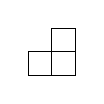
\begin{tikzpicture}
	\draw[] (0,0) rectangle ++(0.3,0.3);
	\draw[] (-0.3,0) rectangle ++(0.3,0.3);
	\draw[] (0,0.3) rectangle ++(0.3,0.3);
\end{tikzpicture}
\hspace{1cm}
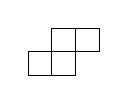
\begin{tikzpicture}
	\draw[] (0,0) rectangle ++(0.3,0.3);
	\draw[] (-0.3,0) rectangle ++(0.3,0.3);
	\draw[] (0,0.3) rectangle ++(0.3,0.3);
	\draw[] (0.3,0.3) rectangle ++(0.3,0.3);
\end{tikzpicture}
\end{center}
\end{figure}

In all the cases above, the temperature is below 3, so it is not a problem. Without losing generality, let \Gm{_1} be a component where there is a right move, and let the initial left move be any such move in \Gm{_1}, therefore, $H^L = G_1^L + G_2$. Now it is clear that this case can be reduced to the case $H = G_*$, with \Gm{_*} a smaller board than \Gm{}:

$$
H^L - H = G_1^L + G_2 - G_1 - G_2 = G_1^L - G_1
$$

Repeating the process with $H = G^L$, $-H = -G^L = -G_1 - G_2$ and $H^L = G_1^L + G_2$. The only cases \Gm{_1^L} does not exist is if
\Gm{=\begin{tikzpicture}
		\draw[] (0,0) rectangle ++(0.3,0.3);
		\draw[] (0.3,0) rectangle ++(0.3,0.3);
	\end{tikzpicture} \text{ or } 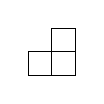
\begin{tikzpicture}
	\draw[] (0,0) rectangle ++(0.3,0.3);
	\draw[] (0.3,0) rectangle ++(0.3,0.3);
	\draw[] (0.3,0.3) rectangle ++(0.3,0.3);
\end{tikzpicture}} and both of them have temperature lesser than 3. Again it is clear that this case can also be reduced to the case $H = G_*$:

$$
H^L - H = G_1^L + G_2 - G_1 - G_2 = G_1^L - G_1
$$

Therefore, if $\ell(G) \leq 3$ then the confusion interval of both option are also smaller than 3. To prove that $G^L - G - 2 \leq 0$ it is shown a winning strategy for right in $G^L - G - 2$, which shows that the position is negative. First notice that $-G$ is \Gm{} flipped so that it fits in a $n\times 2$ board; but a useful way, that is used in this proof, is to consider that $-G$ is Left playing on the horizontal and Right playing on the vertical.

To help visualize the strategy for this case, let the `shadow' of a move be the same cells that the move occupied, but in the opposing board. Also the board resultant from play in $G^L$ is called the original board and the board resultant from play in $-G$ is called the opposing board. For instance:

\begin{figure}[h]
	\centering
	\begin{subfigure}{0.17\linewidth} \centering
		\begin{tikzpicture}
			\node (title) at (0.45,1) {\Gm{^{L/R}}};
			\draw[] (0,0) rectangle ++(0.3,0.3);
			\draw[fill=gray] (0.3,0.3) rectangle ++(0.3,0.3);
			\draw[] (0.6,0.3) rectangle ++(0.3,0.3);
			\draw[fill=gray] (0.3,0) rectangle ++(0.3,0.3);
			\node[] at (1.3,0.3){$\cdots$};
			\node[] at (-0.4,0.3){$\cdots$};
		\end{tikzpicture}
		\caption*{\hspace{0.1cm}Orginal move\newline Original board}
	\end{subfigure}
	\hspace{1cm}
	\begin{subfigure}{0.17\linewidth} \centering
		\begin{tikzpicture}
			\node (title) at (0.45,1) {-$G$};
			\draw[] (0,0) rectangle ++(0.3,0.3);
			\draw[pattern=north west lines,pattern color=gray] (0.3,0.3) rectangle ++(0.3,0.3);
			\draw[] (0.6,0.3) rectangle ++(0.3,0.3);
			\draw[pattern=north west lines,pattern color=gray] (0.3,0) rectangle ++(0.3,0.3);
			\node[] at (1.3,0.3){$\cdots$};
			\node[] at (-0.4,0.3){$\cdots$};
		\end{tikzpicture}
		\caption*{\hspace{0.15cm}Shadow move\newline Opposing board}
	\end{subfigure}
\end{figure}

In the game $G^L -G -2$, if Right plays first, he/she simply has to mimic each and every move Left made by playing the shadow move, maintaining $-2$ intact, starting with the move already played in \Gm{^L}. If, instead Left goes first, he/she can play one of two options. The first is to play a move that does not intersect the shadow of the previous move. In this case, right must play the shadow of either the first or the second move.

Essentially, this first case maintains the original conditions while reducing the board size. This case leads $G^{L_*} -G -2$ to $G^{L_*L} -G^{L_*} -2$, which, by taking $H = G^{L_*}$, is $H^{L} -H -2$. Therefore the only worrisome Left move is one that intersects the shadow of the initial move. This move is not exactly the shadow move because in the opposing board Left moves in another orientation. After Left's move, Right must move on the $-2$ component, taking it to $-1$.

Now, Left can, again, play a move that does not intersect any of the shadows, but this would be met by the same strategy as before, so Left must play a move that intersects a shadow. However, Left cannot move intersecting the shadow of the previous move, because the initial move would be adjacent to this third move and since the mover are both vertical, a $2\times 2$ subgrid would have to exist. The only shadow Left can intersect is that of the first move, playing on the opposing component again. After Left's third move, right plays on the $-1$ component.

At this time, Left can no longer play on any shadows, so he/she cannot avoid Right's strategy and will eventually lose. Therefore, if \Gm{} is a snake fitting in a $2\times n$ grid, then $G^L - G -2 < 0$. This means that $\ell(G),\ell(G^L),\ell(G^R) \leq 2$. By using the bound result, in turn, it means that $t(G) \leq 3$. 

This result from the 2019 paper \cite{12} is different, as stated before, from the 2018 thesis because the first part of the proof, that shows the cases $H=G^L,G^R$ can be reduced to the case $H=G$, was missing. Instead the original text only showed that the confusion intervals of $G^L,G^R$ were smaller than 4. This second result is clear because both $G^L$ and $G^R$ are made of two components that are snakes fitting in $2\times n$ grids. As the text shows that such a snake has the confusion interval smaller or equal to 2, then two snakes have that interval smaller or equal to 4.














